\begin{notecard}{Criterios de congruencia}
    \begin{tcbitemize}[%
            raster columns=4,
            raster equal height,
            raster equal skip=0pt,
            raster column skip=0pt,
            size=small,
            sharpish corners,
            colback=MainColor!2!white,
            colframe=MainColor!50!white,
            colbacktitle=MainColor!20!white,
            center title,
            coltitle=black,
            fonttitle=\small]
        \captionsetup[figure]{labelformat=empty,font={small}}% redefines the caption setup of the figures
        \tcbitem[adjusted title={Lado Lado Lado (LLL)}
        ]
        \begin{figure}[H]
            \centering
            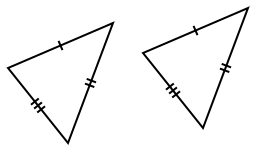
\includegraphics[width=0.9\textwidth]{../images/criterioLLL}
            \caption{Cuando los tres pares de lados correspondientes son congruentes, los triángulos son congruentes.}
            \label{fig:criterioLLL}
        \end{figure}

        \tcbitem[adjusted title={Lado Ángulo Lado (LAL)}]
        \begin{figure}[H]
            \centering
            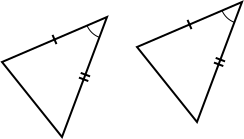
\includegraphics[width=0.9\textwidth]{../images/criterioLAL}
            \caption{Cuando dos pares de lados correspondientes y los ángulos entre ellos son congruentes, los triángulos son congruentes.}
            \label{fig:criterioLAL}
        \end{figure}

        \tcbitem[adjusted title={Ángulo Lado Ángulo (ALA)}]
        \begin{figure}[H]
            \centering
            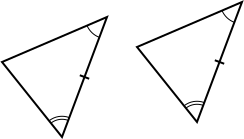
\includegraphics[width=0.9\textwidth]{../images/criterioALA}
            \caption{Cuando dos pares de ángulos correspondientes y los lados entre ellos son congruentes, los triángulos son congruentes.}
            \label{fig:criterioALA}
        \end{figure}

        \tcbitem[adjusted title={Ángulo Ángulo Lado (AAL)}]
        \begin{figure}[H]
            \centering
            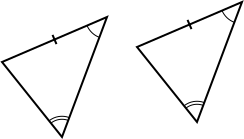
\includegraphics[width=0.9\textwidth]{../images/criterioAAL}
            \caption{Cuando dos pares de ángulos correspondientes y un par de lados correspondientes (no entre los ángulos) son congruentes, los triángulos son congruentes.}
            \label{fig:criterioAAL}
        \end{figure}
    \end{tcbitemize}
\end{notecard}